\begin{frame}
\frametitle{We won!}
% We decided to join although we were both in the money 
% The best decision ever. We had a very good cooperation.
% It took us 2 weeks to fully integrate our solution and
% understand how to use the potential.

% 2.9% relative difference to 2nd team
At the time of merging we were 1st (Konstantin) and 2nd (Pawel).
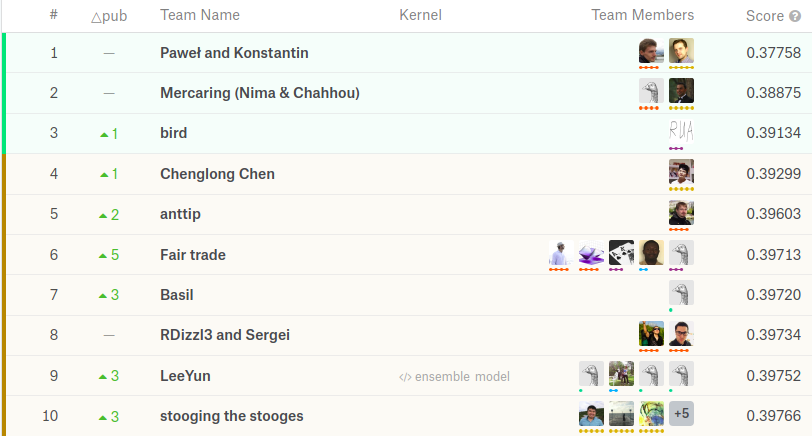
\includegraphics[width=11cm]{img/leaderboard.png}
\end{frame}
 
\begin{frame}
\frametitle{Mercari competition}
% the idea was simple:
% take an item and predict its price given the description, name, category, brand name
% the metric that was used was RMSLE:
% - outliers hurt (if you remove 0.01% of the worst predictions the error improves by 1%)
\href{https://www.kaggle.com/c/mercari-price-suggestion-challenge/}{https://www.kaggle.com/c/mercari-price-suggestion-challenge/}
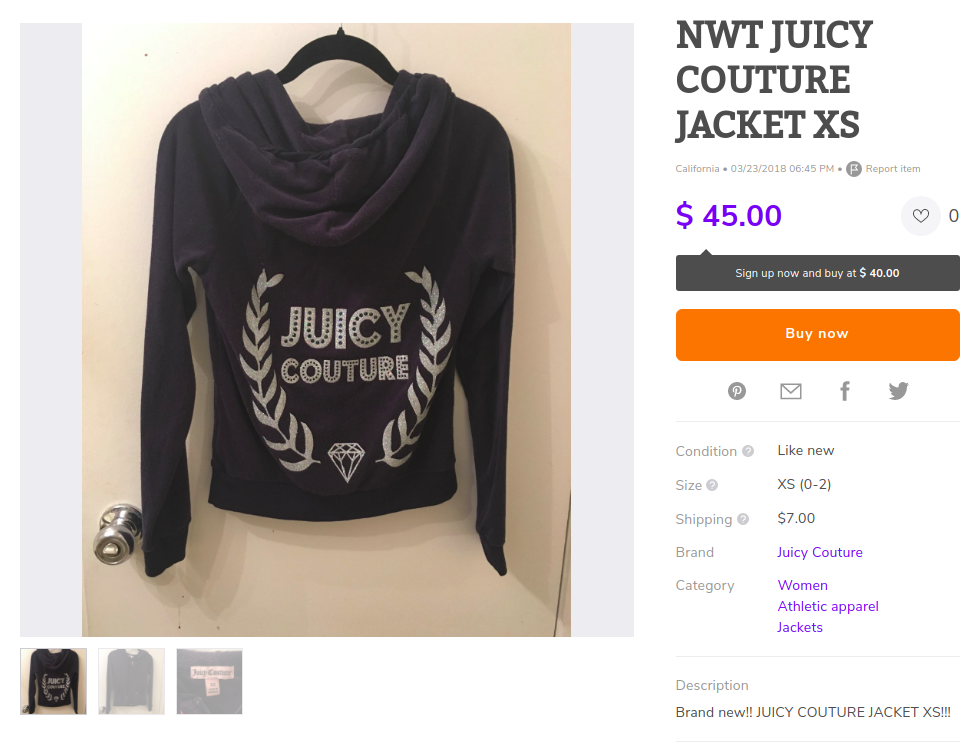
\includegraphics[width=8cm]{img/mercari-item.png}
\end{frame}


\begin{frame}[fragile]
\frametitle{Evaluation RMSLE}

% the evaluation was Root Mean Squared Logarithmic Error
% long name but really when you see something like this
% you want to simplify this

% many algorithms can optimize RMSE so you can convert the target to log and then
% reverse this during the prediction

RMSLE

$$\epsilon = \sqrt{\frac{1}{n} \sum\limits_{i=1}^n (\log(p_i + 1) - \log(a_i+1))^2 }$$

Better to convert to RMSE - optimize directly

\begin{verbatim}
y_log = log(y + 1)
model.fit(X, y_log)
prediction_log = model.predict(X_test)
prediction = exp(prediction_log) - 1
\end{verbatim}

\end{frame}

\begin{frame}
\frametitle{Why Logarithm?}

% why even bother with logarithm
% you can see that when you convert the prices to log(prices)
% it is distribution in a nicer way, also relative errors matter more
% as with any metric that has a square error - outliers matter
% in this competition there were many outliers
% most of which had very sparse description
% bundle items when someone sells not one but many items

Price distribution \\
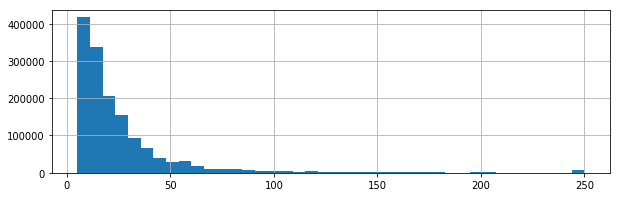
\includegraphics[width=0.75\textwidth]{img/price_distribution.png}

Log(price) distribution \\
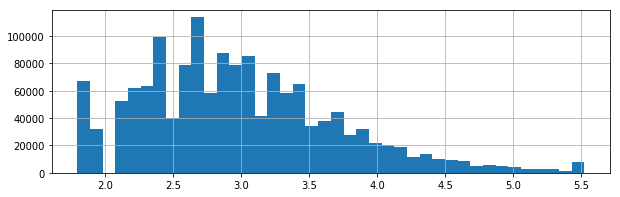
\includegraphics[width=0.75\textwidth]{img/price_log_distribution.png}

\end{frame}

\begin{frame}
\frametitle{Code competition}

%competition was unique and woke me up from retirement

Only 60 minutes to train and predict!

\hfill

System specification: 16 GB ram, 1 GB disk, $\sim4$ cores

\hfill

Advantages
\begin{itemize}
\item No huge ensembles % 6 years on kaggle - tired of creating complex models
\item Team collaboration - common code base % we didn't have 2 solutions - our solution was single
\item Small models, fast iteration
\end{itemize}

Disadvantages
\begin{itemize}
\item Pure optimization % there was a part of this competition which was not related to machine learning
                        % but memory management, dealing with Python multiprocessing (!)
\item Unstable platform % even 10% differences run to run
\item 2 stage competition (5x bigger test data)
\end{itemize}
\end{frame}

\begin{frame}
% code competition - 1 script or notebook 
% 1000 lines+ solution hard to work with
% our code was in a Python package - good maintenance
\frametitle{Build system}
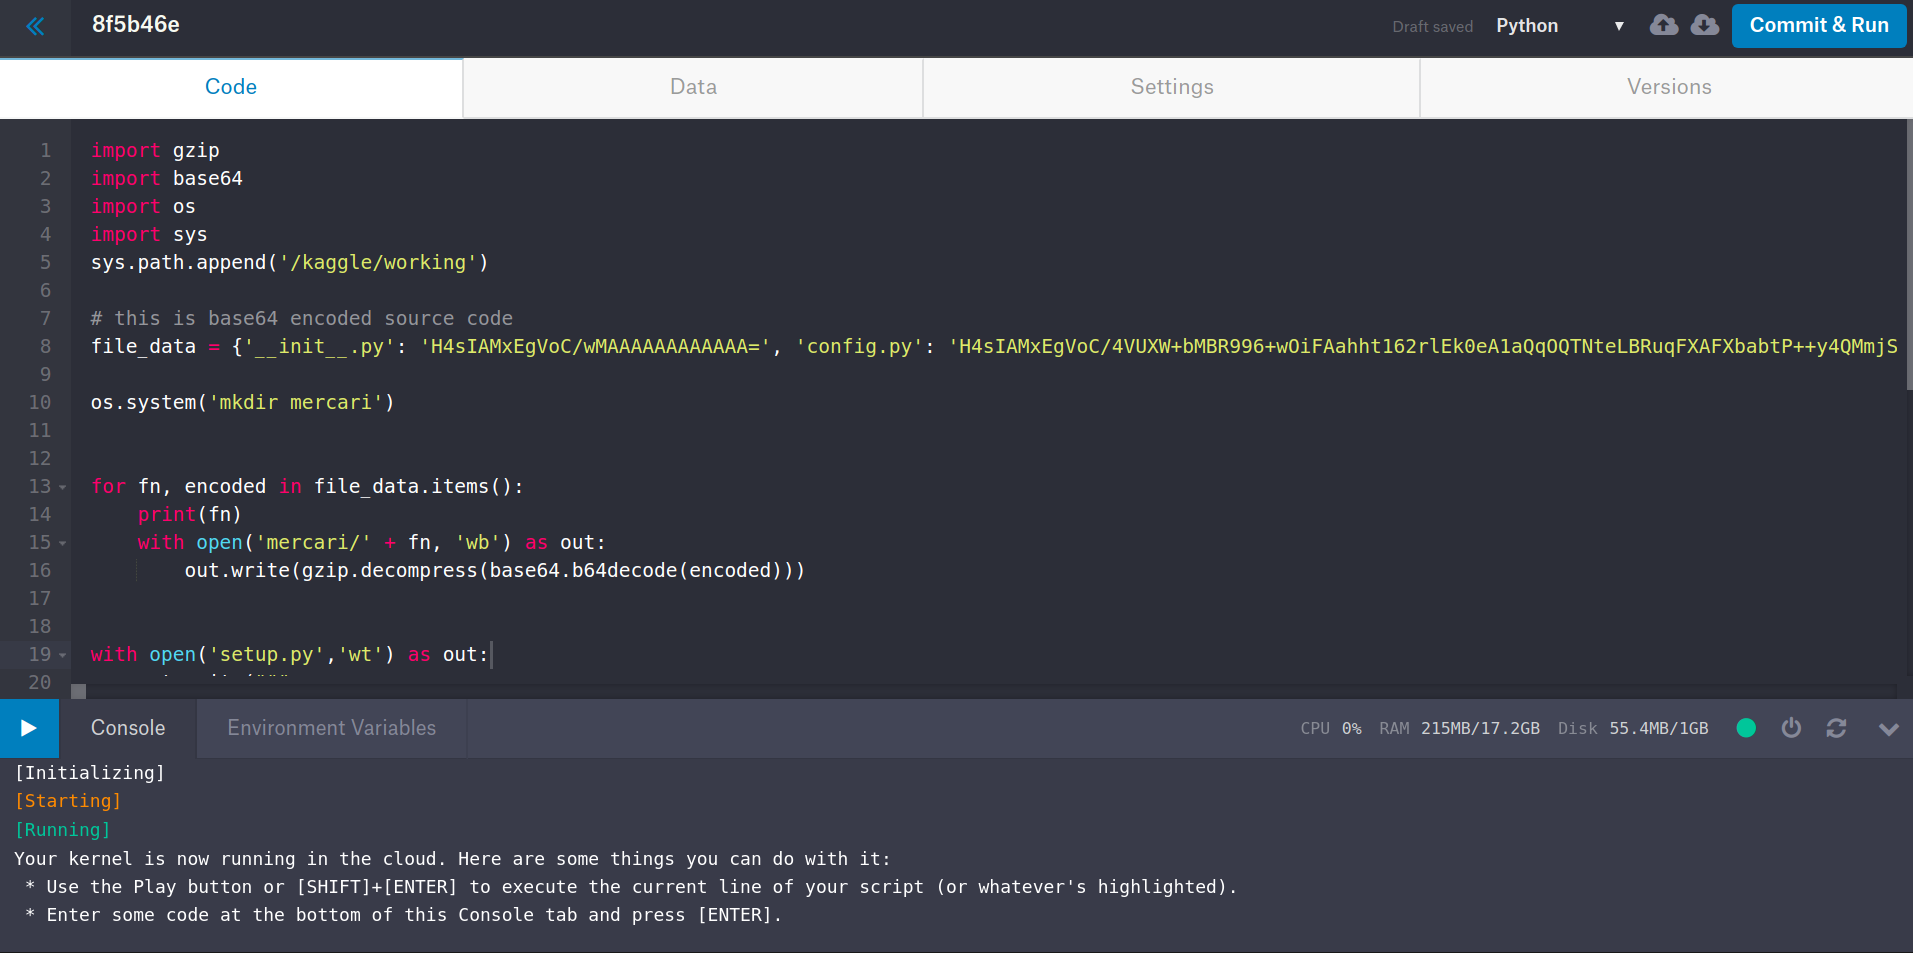
\includegraphics[width=14cm]{img/kernel-code.png}
\end{frame}

\begin{frame}
\frametitle{About the data}

% A few words about the dataset itself.
% I've already said that we didn't have pictures in the dataset
% what we had was 6 columns

1.5 million observations in the training data 

\hfill \break

\begin{tabular}{lll}
Column name & Type & \# unique values \\ \hline
name & text & - \\
item\_description & text & - \\ 
item\_condition\_id & categorical - ordinal & 5 \\
category\_name & text/categorical & 1288 \\
brand\_name & text/categorical & 4810 \\
shipping & boolean & - \\ \hline
\end{tabular}
\end{frame}


\begin{frame}
\frametitle{Example Item}
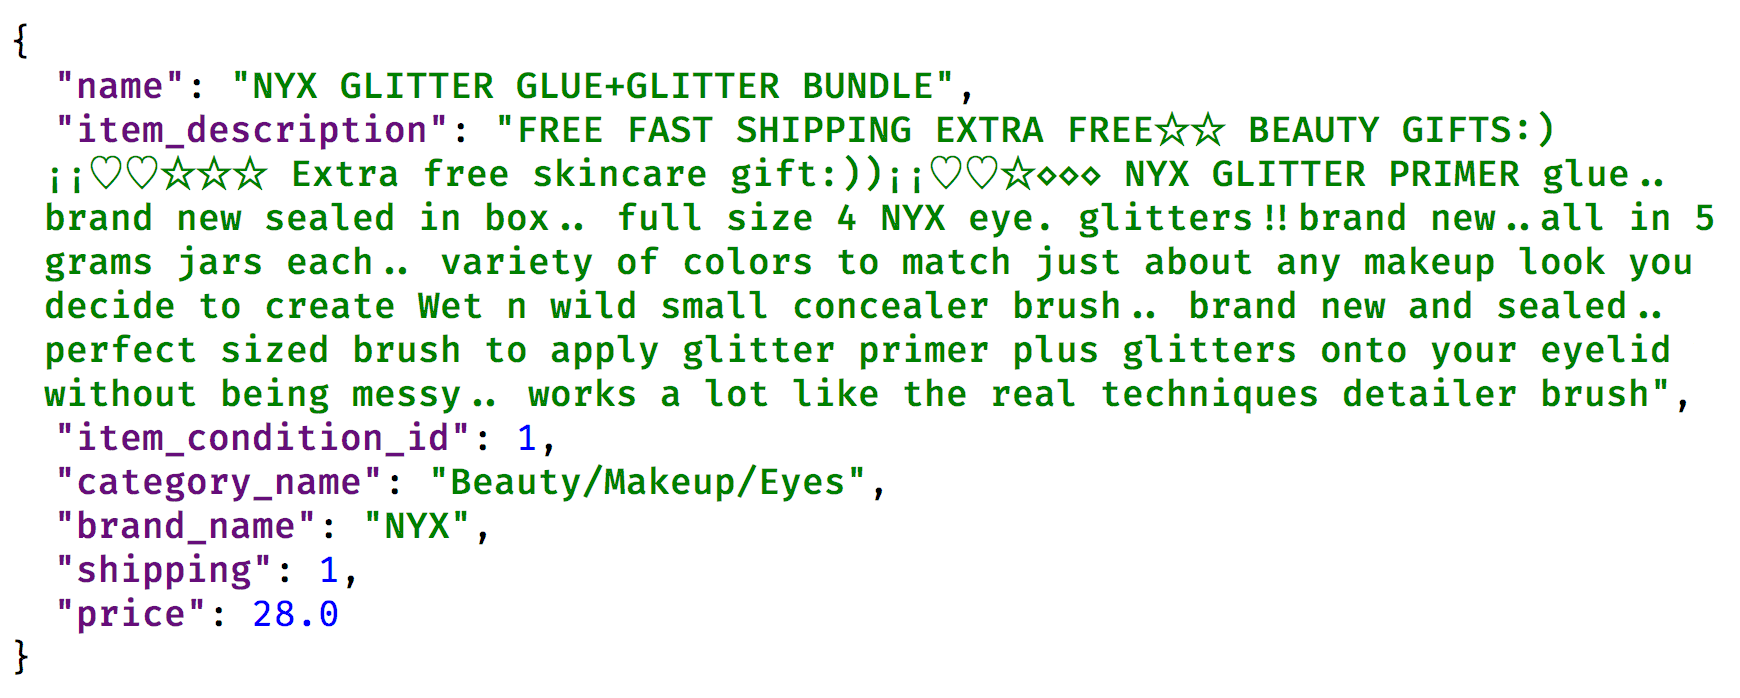
\includegraphics[width=14cm]{img/data_sample.png}
\end{frame}
